%----------------------------------------------------------------------------------------
%	DOCUMENT CONFIGURATIONS
%----------------------------------------------------------------------------------------

\documentclass[]{article}

\usepackage{graphicx} % To include figures
\usepackage[utf8]{inputenc}
\usepackage{fancyhdr} % Required for custom headers
\usepackage{lastpage} % Required to determine the last page for the footer
\usepackage{extramarks} % Required for headers and footers
\usepackage[a4paper, top=4cm, bottom=4cm, left=3.3cm, right=3.2cm]{geometry}
%for the bibliography
\usepackage{booktabs}
\usepackage{url}
\usepackage{tocloft}

\renewcommand{\baselinestretch}{1.5}

% Set up the header and footer
\pagestyle{fancy}
\lhead{Carlos Pérez López} % Top left header
%\chead{\hmwkClass\ (\hmwkClassInstructor\ \hmwkClassTime): \hmwkTitle} % Top center header
\rhead{ASD Assignment: 3D Game} % Top right header
%\lfoot{\lastxmark} % Bottom left footer
%\cfoot{} % Bottom center footer
\rfoot{Page\ \thepage\ of\ \pageref{LastPage}} % Bottom right footer
\renewcommand\headrulewidth{0.4pt} % Size of the header rule
\renewcommand\footrulewidth{0.4pt} % Size of the footer rule


\title{
\vspace{2in}
\textmd{\textbf{ASD Assignment: 3D Game}}\\
\vspace{0.1in}
{\today}\\
\vspace{3in}
}

\author{\textbf{Carlos Pérez López}}
\date{}

\begin{document}

\maketitle % Insert the title, author and date

% If you wish to include an abstract, uncomment the lines below
% \begin{abstract}
% Abstract text
% \end{abstract}

\setlength\parindent{24pt} % Removes all indentation from paragraphs

\renewcommand{\labelenumi}{\alph{enumi}.} % Make numbering in the enumerate environment by letter rather than number (e.g. section 6)
\renewcommand{\cftsecleader}{\cftdotfill{\cftdotsep}}

\newpage
\tableofcontents
\newpage


%----------------------------------------------------------------------------------------
%	SECTION 1
%----------------------------------------------------------------------------------------

\section{Initial Research}

Among all the options for the ASD assignment, the simple 3D video game was chosen. The author found all of them of real interest, but two reasons led him to take that decision. 
The first one is his unfamiliarity with the CGI field; even though he counts with a quite solid basis in computer engineering, all the concepts such as shader, raytracer, renderer, 
flocking system, etc. are new for him. Thus, instead of a more specific project, it was thought that at the same time lectures give a more theorical vision of computer graphics, 
a simple 3D game might be a good choice to get familiar with all of it and adquire a more global vision. And independently of the academic aims, the second reason was a quite well-formed 
idea of a 3D game in the author's mind.

By the time of starting the research, different videos of some 3D games were watched as well as reading the documentation of some libraries commonly used in the field of 
video game programming. Although Qt offers a very complete API, is more focused to the development of applications which need a powerful and friendly GUI. On the other hand, SDL offers 
funtionalities more suitable referring to game programming. The SDL library \cite{sdl} is completely compatible with 3D harware acceleration via OpenGL, and provides a series of strong subsystems
 such as input events, threads, timers, audio, etc. Other of the main advantages of this library are that it supports the use of joysticks, which is really convenient in the world of videogames,
 it is cross-platform and completely open source.
 
 Some other libraries were studied for their use as well. BulletPhysics \cite{bulletPhysics} was thought in first instance as main physics engine to handle the collisions in the world of the game
 due to it is a full package which offers a wide range of collisions detection. In the same way, to implement the AI of the system, the author had in mind OpenSteer \cite{openSteer}, which offers
 steering behaviours for autonomous characters in game and animation. Finally, due to the simplicity of this project both libraries were rejected. Besides, using directly
 low level C++ to implement it, the approach of the used algorithms would be greater, so it would be a better chance to learn.
 
 The final technologies chosen to implement the game were NGL, the graphic library of the NCCA, and SDL2 for handling the graphic context and user events. Later, SDL2\_ttf would also be
 added for debugging purpose and because of some functionalities of rendering text are required at some points of the gameplay.
 
 The main source of learning NGL was the ASD professor website \cite{maceyWebsite} as well as his blog \cite{maceyBlog}. Reading the demos' code and writing small programs was the process of understanding the concepts a progressing 
 little by little. The same happened with SDL, but extending it with all the other sources that might be found through the internet.
 
 Parallel to this, other research was being carried out relative to the design of the game which, certainly, is completely independent of the technologies chosen to implement it. M. Sanchez provided
 to the author the contact of E. Anderson, an experienced teacher in game programming working at BU at the moment. He gently gave to the author an explanation of the typical game architecture, as well as provided 
 some slides he often uses during his lectures.
 
 At this point, the research material and documentation was enough to start with the design of the 3D game.

 
%----------------------------------------------------------------------------------------
%	SECTION 2
%----------------------------------------------------------------------------------------

\section{Initial Design}

Currently, the most part of applications are desgined using the paradigm of Object Orientation, due to the flexibility and scalability that design patterns offer, as well as it is widely belief
as a very smart way of programming. But concerning to this project, it must be said that the execution of a game is normally a very secuencial flow.

All the games has a main loop with a similar estructure:
\begin{itemize}
 \item reading the player input
 \item updating the world
 \item checking the collisions
 \item drawing the world
 \item adjusting FPS
\end{itemize}

So to design this execution flow, it was decided to count with a class \emph{GameManager} which will be the centre of the system and will mantain the specific behaviour of this specific game. 
The rest of the modules which are surrounding this master class will purely have an object oriented design and will conform our game engine. See \ref{fig:ge}.

\begin{figure}[h]
\begin{center}
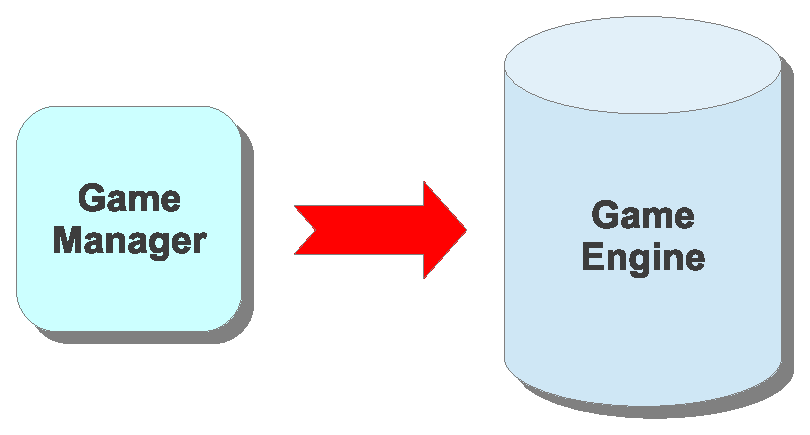
\includegraphics[width=0.5\textwidth]{images/gameEngine.eps}
\caption{Game engine scheme}
\label{fig:ge}
\end{center}
\end{figure}

A game engine is a framework designed for the creation and development of video games. It might be thought as a group of predefined functions that offer to the game developper behaviour
already programmed. Thus, all the different modules in this game should be part of a game engine, the most independent possible of this specific game, and that might be used in the future by
other games of similar characteristics.

Once these concepts were clarified and the main structure was decided, the different modules had to be thought. Some of the main worries of the author at the time of the design were the flexibility
and the scalability, so a convenient idea was treat every module as an independent system which is in charge of certain responsabilities logically grouped and that could be unacoplated and used by any
other client. 

In order to model the world, a class \emph{Object} was defined, which represents a simple object in the world and that mainly stores state information and some little behaviour for the interaction
with other objects. This is the top of the hierarchy, and then some other classes with more specific state and behaviour might be defined. To store the objects of a concrete world there is a manager
named \emph{ObjectManager} which holds a list with all the objects and provides an interface with basic operations such as \emph{addObject} or others more linked to this context.

The module in charge of updating the world is born in the class \emph{Controller}, which provides a hierarchy of different autonomous behaviours (the AI of the game) as well as the controller defined
by the user input. At first, this was thought as a strategy pattern, since the objects might have different strategies of movement but later, regarding the fact that is the controller the entity
that moves an object and will have to modify its state, it was decided to use composition. So, in the same way, we count with a manager class that deals with all the controllers in order to give 
the client abstraction and to avoid they manage each one of them manually. The figure \ref{fig:object-controller} shows this.

\begin{figure}[h]
\begin{center}
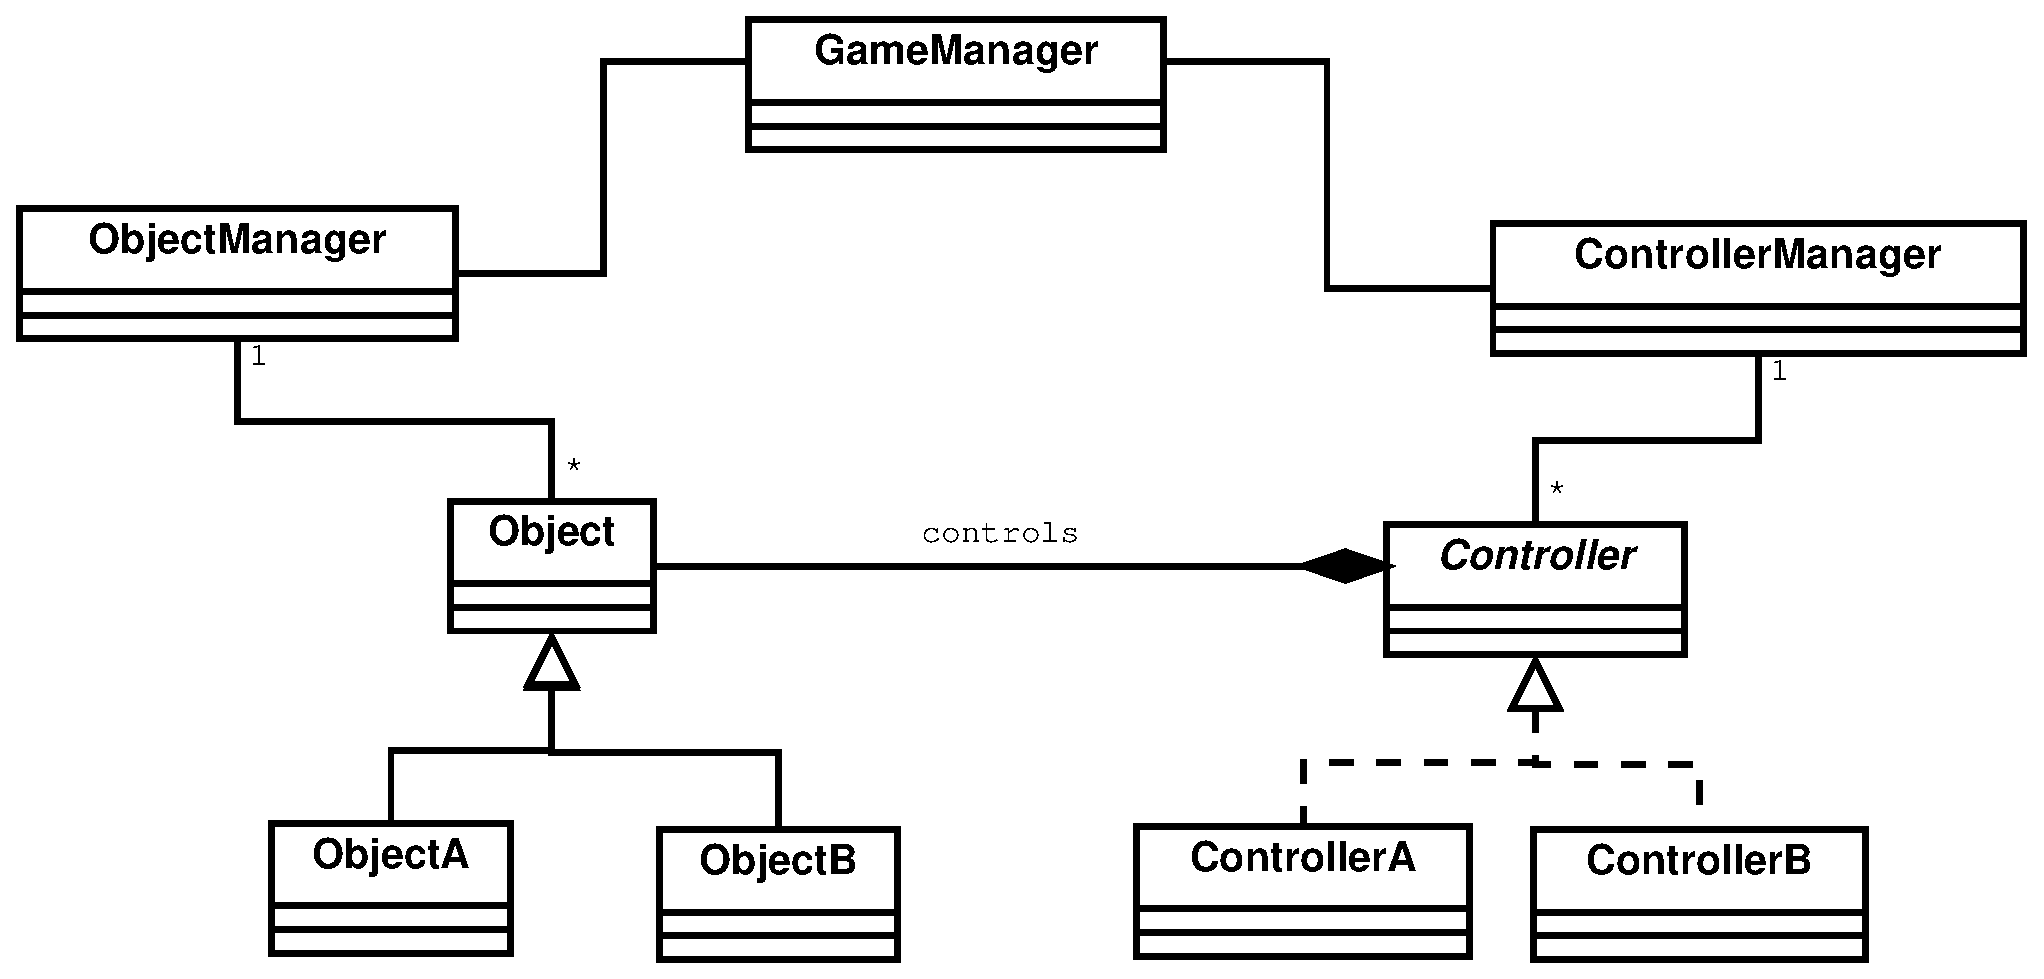
\includegraphics[width=0.75\textwidth]{images/object-controller.eps}
\caption{Controller-Object composition}
\label{fig:object-controller}
\end{center}
\end{figure}

One of the critical points of computer games is the check of collisions among the objects moving around the world. In this approach, it was decided that the best option is that the responsability
of checking the collisions should be carried out by the holder of the objects but, using a phyics engine object provided by the client. The \emph{ObjectManager} just deals with a \emph{PhysicsEngine}
object which in this system is an abstract class and might be thought as an interface whose implementation depends on the specific physics engine used. In this way, this design provides a very high
flexibility. See \ref{fig:pesec}.

\begin{figure}[h]
\begin{center}
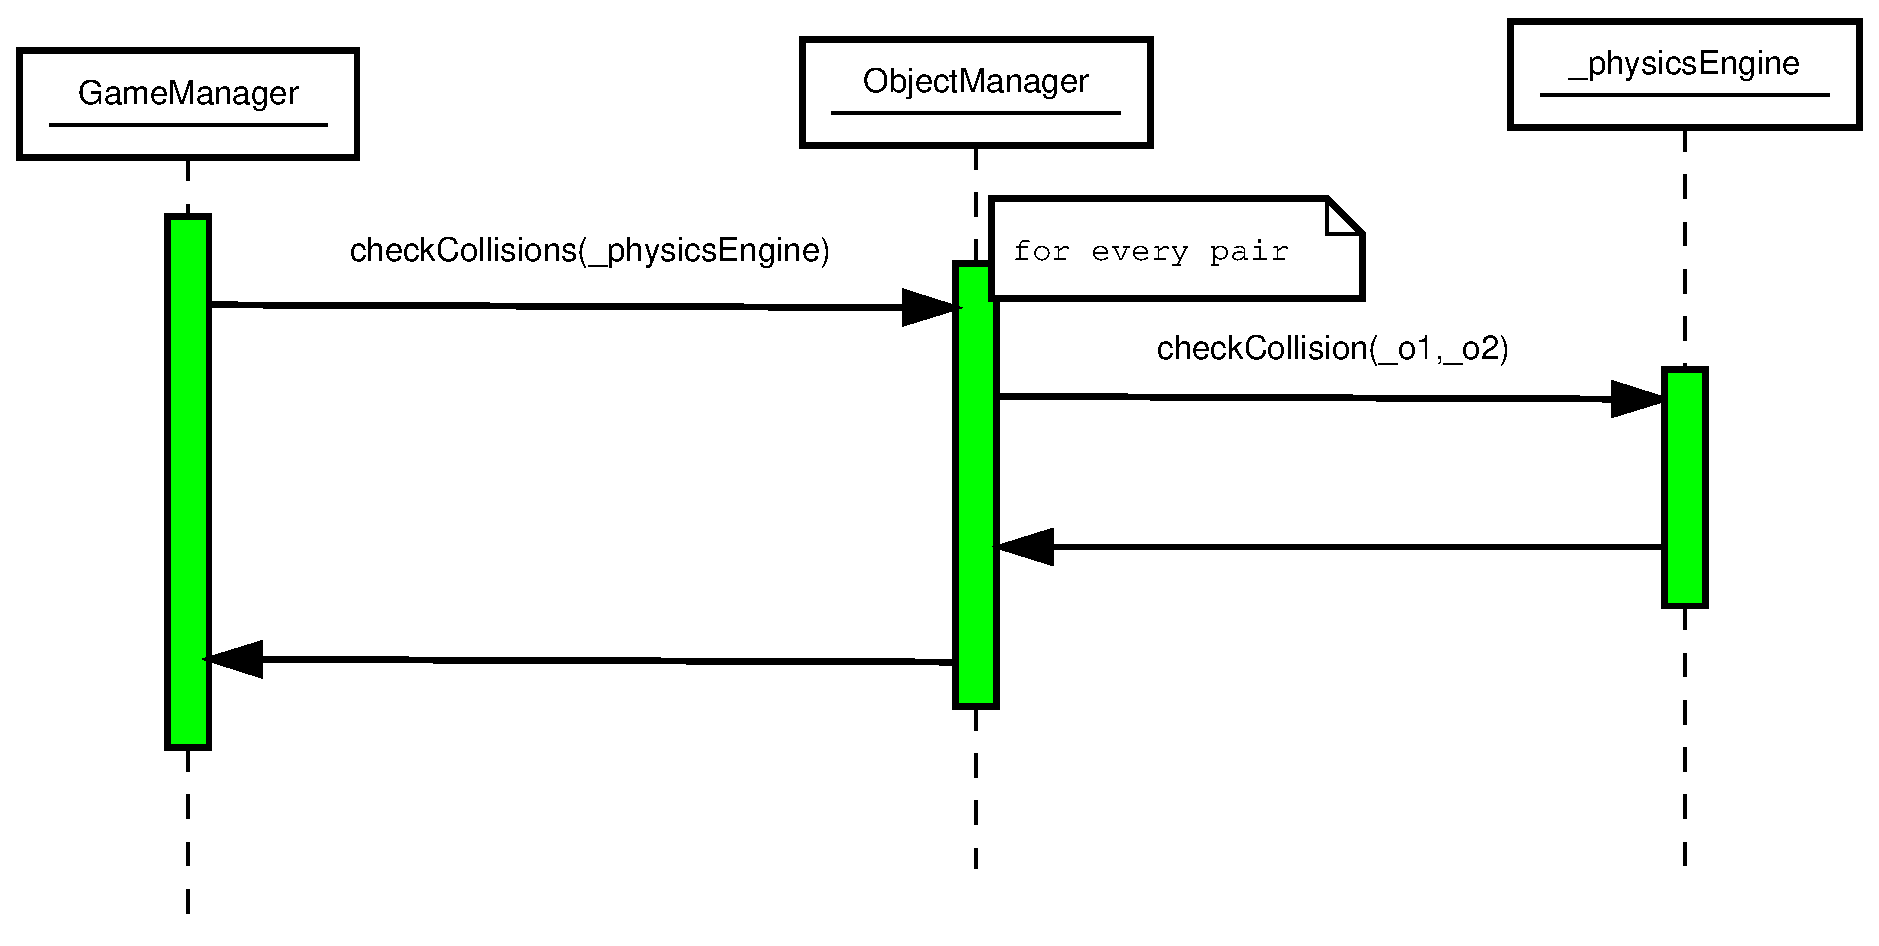
\includegraphics[width=0.75\textwidth]{images/physicsEngineSec.eps}
\caption{Sequence of the collisions check}
\label{fig:pesec}
\end{center}
\end{figure}

Concerning to the graphic module of this assignment, which is one of great importance taking into account the nature of this course itself, there is a class that is in charge of all the funtionalities
related with the drawing, which could not be named in other way that \emph{Renderer}. The \emph{Renderer} is the responsible of creating the graphic context and initialize everything needed for the
rendering of the current scene of the game's world. It deals with the shaders and lights, and it is thought to be able to draw any 3D object over a background as well as 2D images or text. At the time 
the client asks for the render of the world, they should provide a reference to the world and its background, the camera from where the render should be processed and a simple flag to indicate a \emph{debugMode}.
As a design decision, the cameras are treated apart and independently to offer the user more transparency and versatility to visualize the scene. A \emph{CameraManager} is added to the design as well to
update all the positions of the different type of cameras according with a target, that is the main object of the world, the one the player is controlling.

The design counts with a class which acts as a stock and stores all the sources needed for the execution of our game, such as meshes, textures, images, text, sound, etc. This is the 
\emph{SourceManager}. The presence of managers is quite abundant in this system, the reason is that there will be a big amount of different objects during the runtime, and they can offer abstraction
to the \emph{GameManager} to deal with all of them. At first it was thought to make them singletons, but finally it was taken the option of just keeping one single instance of each manager.

Finally, in order to load our game world, a \emph{Parser} is used to read from a describing scene file and some auxiliar functions used by the \emph{GameManager} were grouped in a \emph{Utilities} class.

A diagram of sequence is shown in \ref{fig:mainLoop} to illustrate how the main loop works and how the \emph{GamaManager} interacts with the different modules.

\begin{figure}[h]
\begin{center}
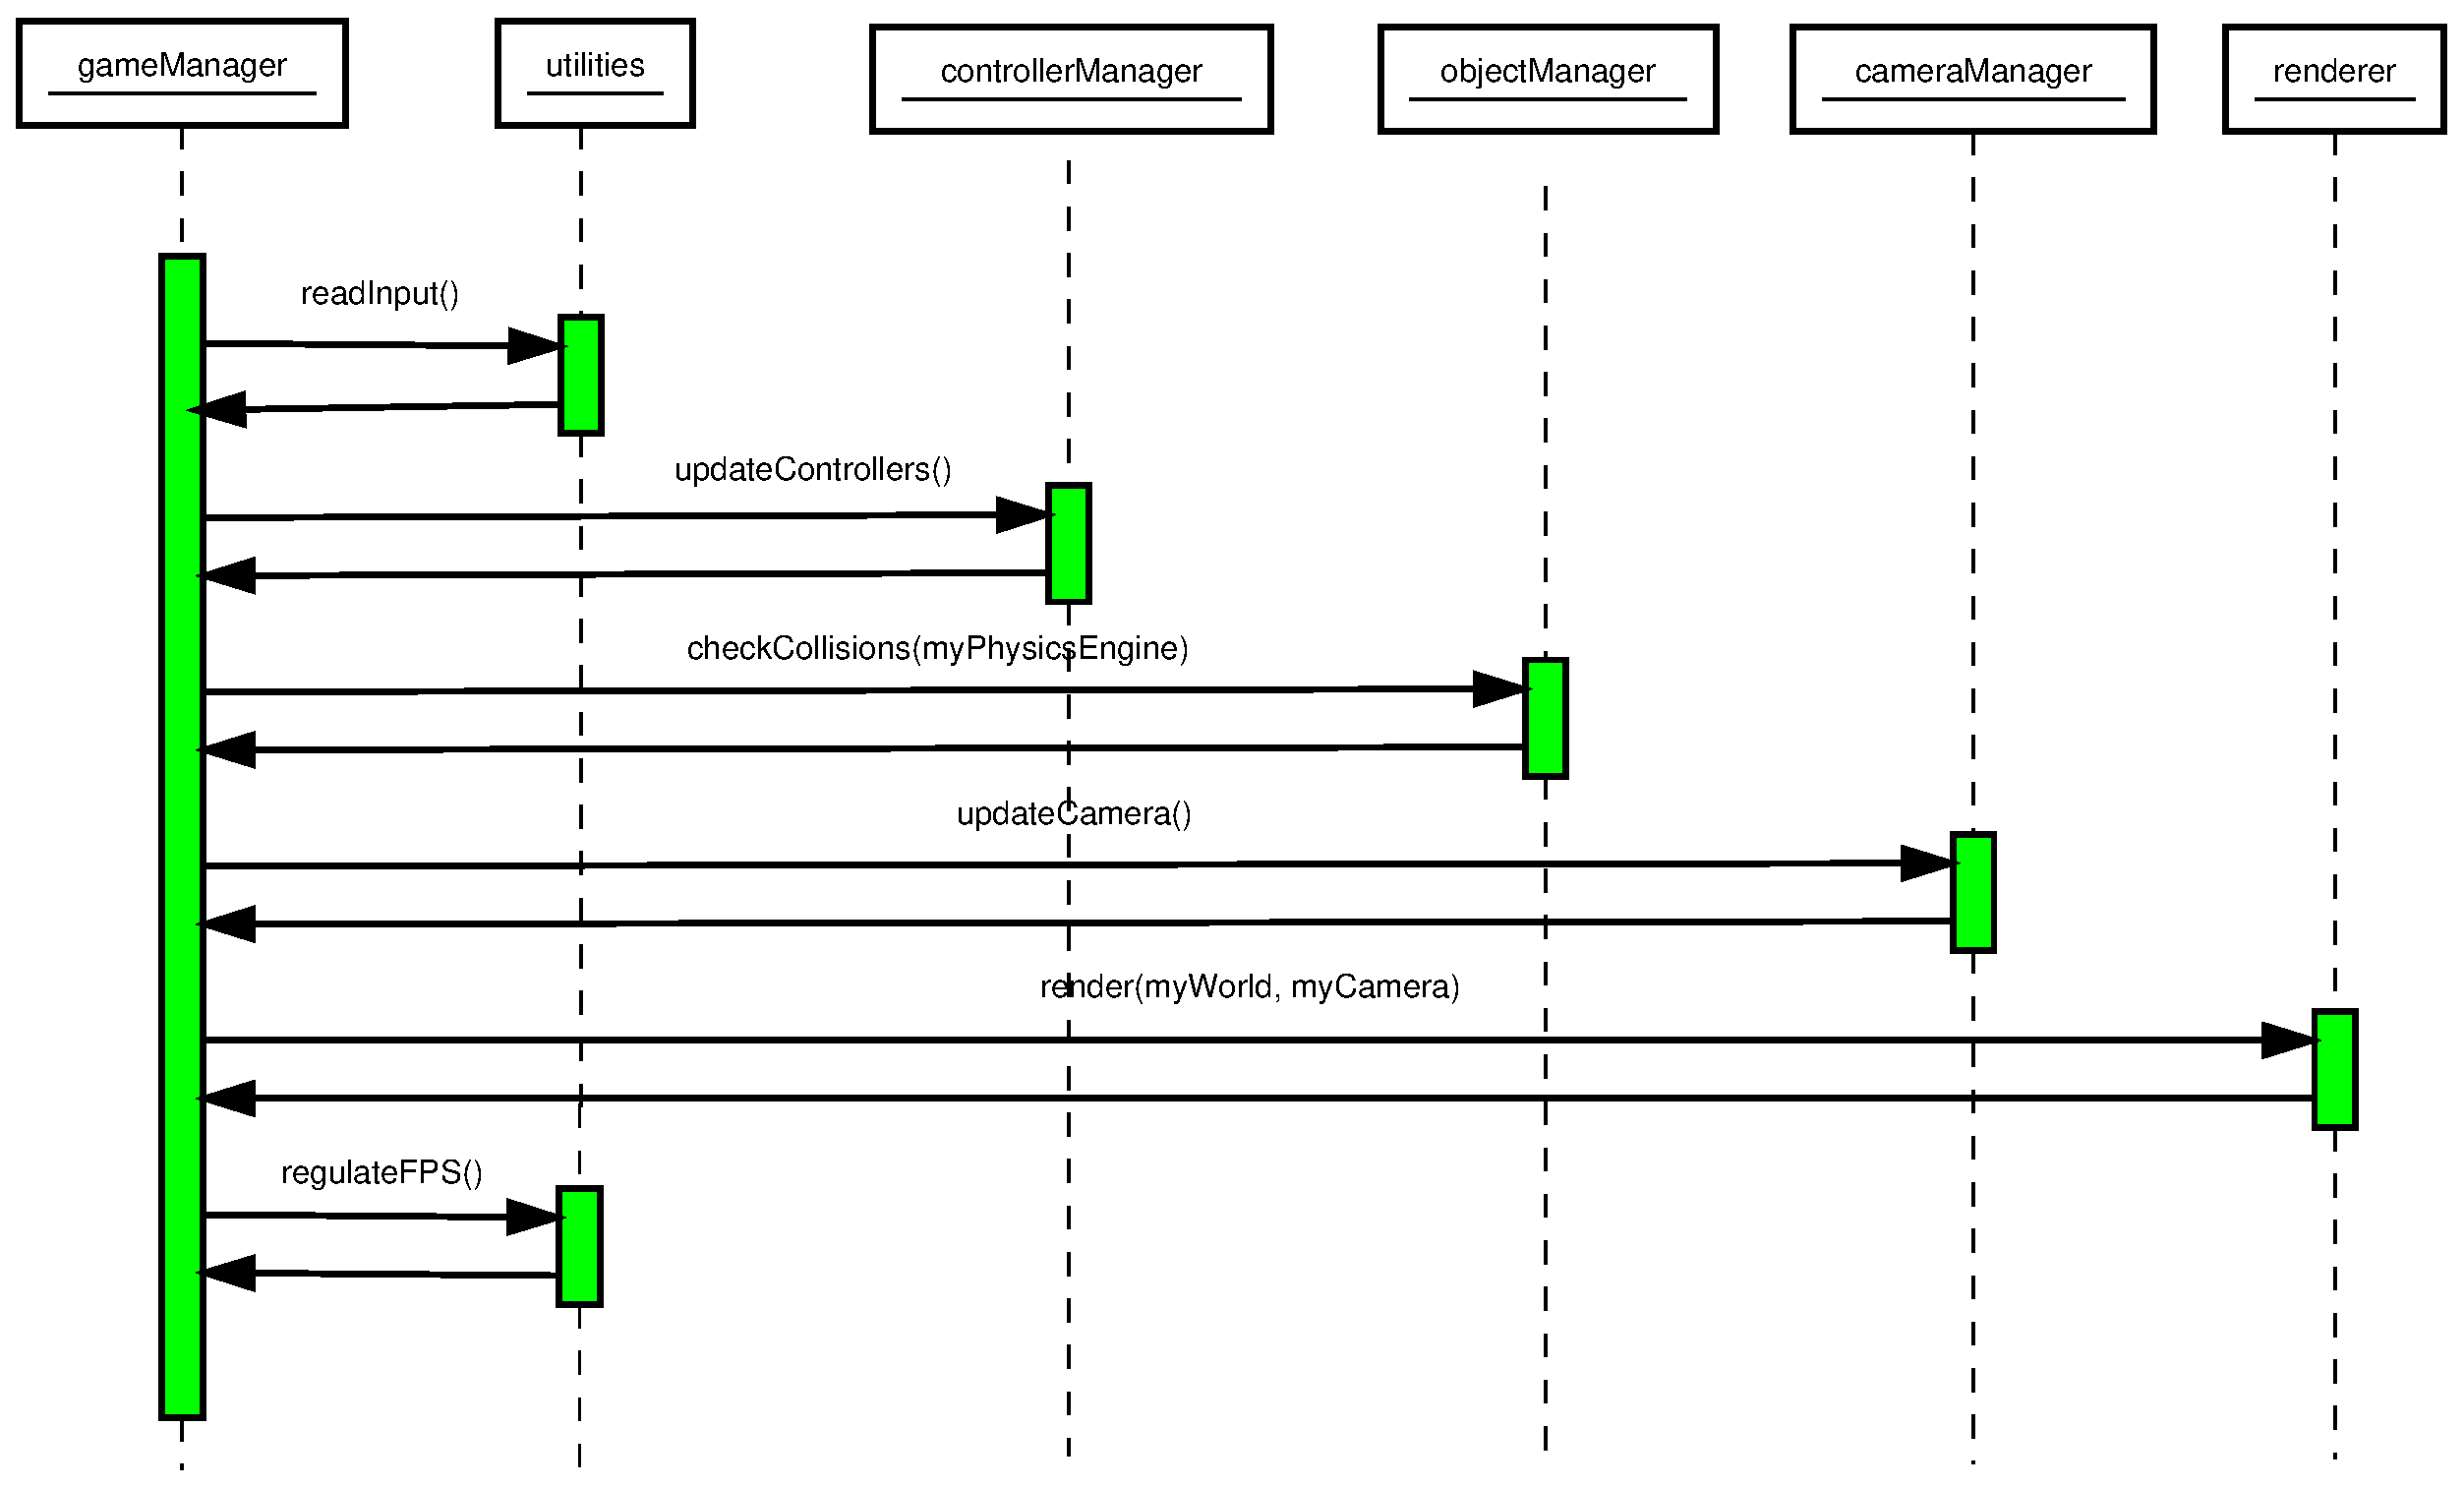
\includegraphics[width=1\textwidth]{images/mainLoopSequence.eps}
\caption{Sequence of the main loop}
\label{fig:mainLoop}
\end{center}
\end{figure}

%----------------------------------------------------------------------------------------
%	SECTION 3
%----------------------------------------------------------------------------------------

\section{Proof of Context}

The main aim of this first approach is the design, but a simple prototype is attached as a proof of context. The developer has a programming background in java an C, thus there is a period of adaptation to C++ 11, so one of the main objects of this prototype is getting familiar to this technology.

This first version of the application shows the gameplay, rendered on a openGL context using NGL and SDL. So far it is single player and keyboard controlled, by this is tied to future modifications presented in the next section. The user will control an object which will be the main character of the world.

All the world is ambiented at the sea, so, in this context, the generic objects might perform roles such as obstacles on the sea, different types of boats or even marine fauna. The aim of the game is reaching the beach, which is at the end of the track where the main speedboat is advancing on. The main idea, which is not already implemented, is that the player might loose the game in two situtations; if he looses all the load in his speedboat or if the police boats catch him. All of this is linked to the game story which is not relevant for this technical part.

It might be noticed that the AI is a very wide field to work when we are talking about boats moving on the sea, where a good understanding of physics plays a really important role. Some basic but different behaviours methods were implemented, thus the player might find boats which are crossing the sea track, which are coming towards the speedboat, etc. 

The prototype can work so far with some test meshes and in two different debugging modes:

\begin{itemize}
\item mode 1: this is the primitives mode, where all the objects are rendered as primitives and the velocity vectors are drawn.
\item mode 2: this is the collision mode, where the bounding spheres are rendered showing when a collision is produced.
\end{itemize}

It is possible to access to a specific debugging mode pressing the corresponding key number. For no debugging mode press 0.

The set of default cameras offered to the user for the rendering of the game scene is loaded at the initialization of the game. There is a circular queue of cameras which holds the typical cameras present on a video game, such as the camera from the back, up camera or first person camera. To iterate over this set of cameras the key \emph{c} must be pressed. In addition, it was added a special camera, the back camera, which will be active while the player press \emph{backspace}. The purpose of this camera for the real game is that it might be a useful feature when the police is chasing the player.

Other test functionalites have been added as well. It is possible to pause the game with the key \emph{pause} or to interact with the window changing its size or converting it to fullscreen mode.


%----------------------------------------------------------------------------------------
%	SECTION 4
%----------------------------------------------------------------------------------------

\section{Future work}

This prototype compounds the main core of the game a it is thought to be formed by different modules the most indepent possible. In this way, the application will adquire a flexible and scalable architecture profitable for reusability and expansibility.

After this first version, some reflexions were taken and some hints for future work and improvements on the system in the next term are these:

\begin{itemize}
\item Adding a Game State pattern to the design to manage the different states of the game, such as menu, story level, scores or gameplay.
\item Adding the \emph{Checkpoint} feature perhaps with a memento pattern.
\item As it is a game about boats, it was considered a good idea to add particles systems to simulate the interaction of the motors or the hulls against the sea water.
\item Improving the \emph{physicsEngine} and the quality of the collision detection.
\item Adding a subsystem of radio conversations. The player will be able to see on the screen radio conversations (rendering images and text) which in some situations might work as tutorial guide, information, story or a gag launched by some event in the gameplay. The first idea to desigh this is using an observer-observable pattern between the radio conversations and the objects, so every object can notify to a \emph{ConversationManager} when a collision takes place.
\item Adding a new controller to support the use of a joystick such as a play-station joystick.
\item Once the engine and technical part are finished, work on the visual impact of the game to make it atractive. Model good looking meshes and work on the appearence, thus it is a very important part of a 3D game.
\end{itemize}

\newpage

%----------------------------------------------------------------------------------------
%	BIBLIOGRAPHY
%----------------------------------------------------------------------------------------

\bibliographystyle{apalike}

\begin{thebibliography}{}

\bibitem[SDL 2.0, 2012]{sdl}
Lantinga, S (2012).
\newblock Available on:
  \url{http://wiki.libsdl.org/moin.cgi}
\newblock Accessed \today.

\bibitem[BulletPhysics, 2012]{bulletPhysics}
\newblock Available on:
  \url{http://bulletphysics.org/wordpress}
\newblock Accessed \today.

\bibitem[OpenSteer, 2012]{openSteer}
\newblock Available on:
  \url{http://opensteer.sourceforge.net}
\newblock Accessed \today.

\bibitem[J. Macey's website, 2012]{maceyWebsite}
Macey, J (2012)
\newblock Available on:
  \url{http://nccastaff.bournemouth.ac.uk/jmacey}
\newblock Accessed \today.

\bibitem[J. Macey's blog, 2012]{maceyBlog}
Macey, J (2012)
\newblock Available on:
  \url{http://jonmacey.blogspot.co.uk}
\newblock Accessed \today.

\end{thebibliography}

\end{document}
